\documentclass{article}

\usepackage{tikz}
\usetikzlibrary{shapes.geometric, arrows}

\tikzstyle{startstop} = [
    rectangle,
    rounded corners,
    minimum width = 3cm,
    minimum height = 1cm,
    text centered,
    draw = black,
    fill = red!30
]

\tikzstyle{inbetween} = [
    rectangle,
    rounded corners,
    minimum width = 3cm,
    minimum height = 1cm,
    text centered,
    draw = black,
    fill = white!30
]

\tikzstyle{arrow} = [thick, ->, >=stealth]

\begin{document}

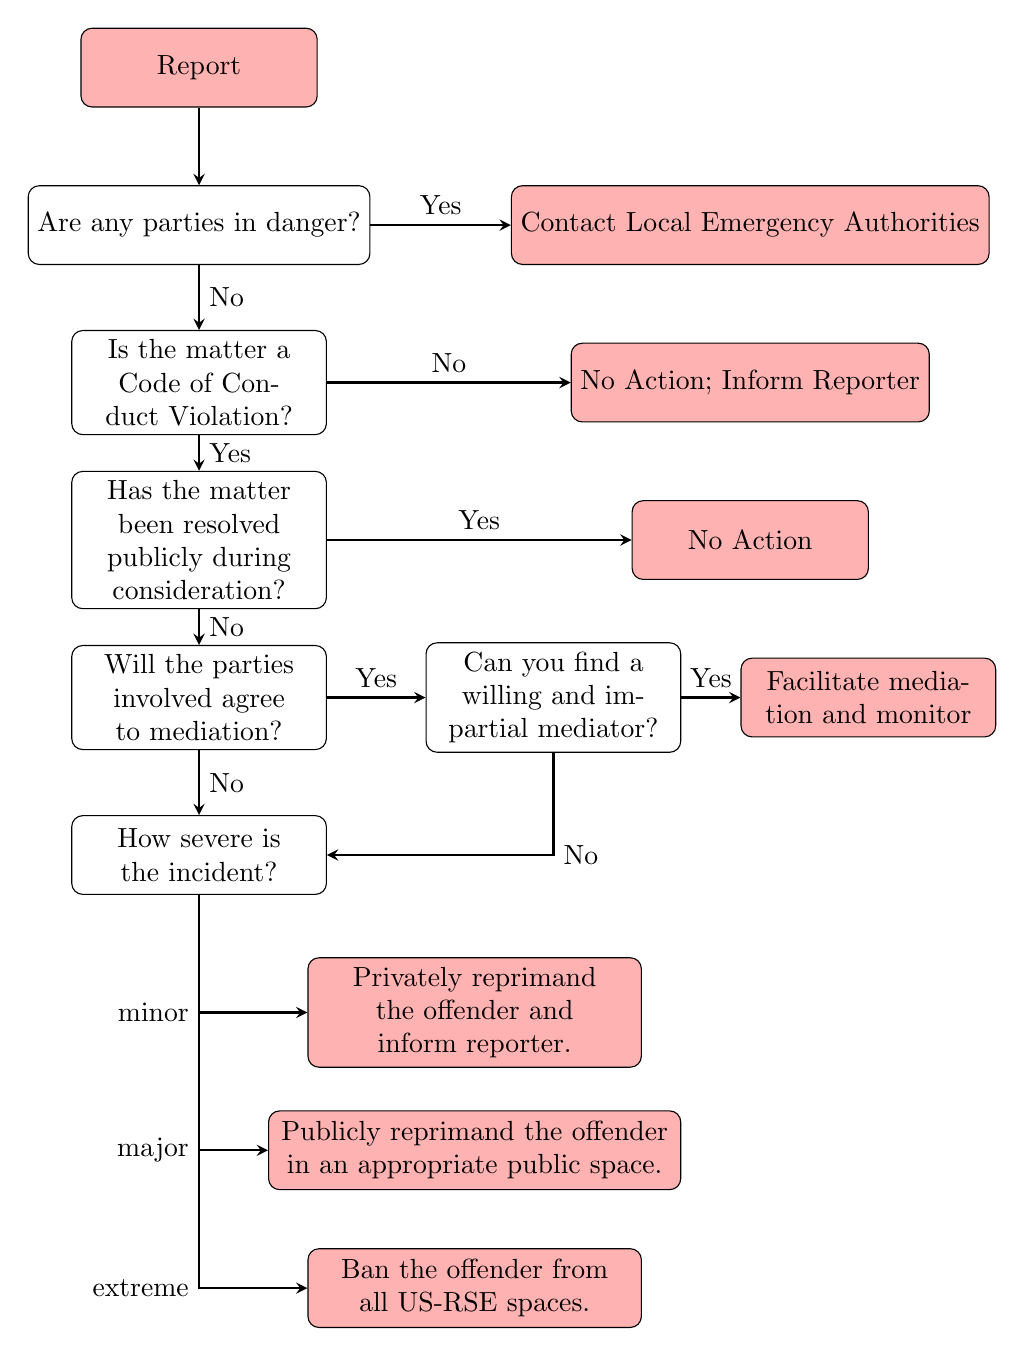
\begin{tikzpicture}[node distance = 2cm]
    \node (report) [startstop]{Report};


    \node (danger) [inbetween, below of = report]
        {Are any parties in danger?};

    \draw [arrow] (report) -- (danger);

    \node 
        (contact authorities)
        [startstop, right of = danger, xshift = 5cm]
        {Contact Local Emergency Authorities};

    \node
        (determine violation)
        [inbetween, below of = danger, text width = 3cm]
        {Is the matter a Code of Conduct Violation?};

    \draw [arrow] 
        (danger) -- node[anchor=south]{Yes}(contact authorities);

    \draw [arrow]
        (danger) -- node[anchor=west]{No}(determine violation);

    \node
        (not violation)
        [startstop, right of = determine violation, xshift = 5cm]
        {No Action; Inform Reporter};

    \node
        (matter resolved)
        [inbetween, below of = determine violation, text width = 3cm]
        {Has the matter been resolved publicly during consideration?};


    \draw [arrow]
        (determine violation) --
        node[anchor=south]{No}(not violation);

    \draw [arrow]
        (determine violation) --
        node[anchor=west]{Yes}(matter resolved);

    \node
        (resolved)
        [startstop, right of = matter resolved, xshift = 5cm]
        {No Action};

    \node
        (mediation)
        [inbetween, below of = matter resolved, text width = 3cm]
        {Will the parties involved agree to mediation?};

    \draw [arrow]
        (matter resolved) --
        node[anchor=south]{Yes}(resolved);

    \draw [arrow]
        (matter resolved) --
        node[anchor=west]{No}(mediation);

    \node
        (find mediator)
        [inbetween, right of = mediation, text width = 3cm, xshift = 2.5cm]
        {Can you find a willing and impartial mediator?};

    \draw [arrow]
        (mediation) --
        node[anchor=south]{Yes}(find mediator);

    \node
        (found mediator)
        [
            startstop,
            right of = find mediator, text width = 3cm, xshift = 2cm
        ]
        {Facilitate mediation and monitor};

    \draw [arrow]
        (find mediator) --
        node[anchor=south]{Yes}(found mediator);

    \node
        (incident severity)
        [inbetween, below of = mediation, text width = 3cm]
        {How severe is the incident?};

    \draw[arrow]
        (mediation) --
        node[anchor=west]{No}(incident severity);

    \draw[arrow]
        (find mediator) |-
        node[anchor=west]{No}(incident severity);

    \node
        (private reprimand)
        [
            startstop,
            below of = incident severity,
            text width = 4cm,
            xshift = 3.5cm,
        ]
        {
            Privately reprimand the offender and inform reporter.
        };

    \draw[arrow]
        (incident severity) |-
        node[anchor=east]{minor}(private reprimand);

    \node
        (public reprimand)
        [
            startstop,
            below of = incident severity,
            text width = 5cm,
            xshift = 3.5cm,
            yshift = -1.75cm,
        ]
        {
            Publicly reprimand the offender in an appropriate public space.
        };

    \draw[arrow]
        (incident severity) |-
        node[anchor=east]{major}(public reprimand);

    \node
        (ban)
        [
            startstop,
            below of = incident severity,
            text width = 4cm,
            xshift = 3.5cm,
            yshift = -3.5cm
        ]
        {
            Ban the offender from all US-RSE spaces.
        };

    \draw[arrow]
        (incident severity) |-
        node[anchor=east]{extreme}(ban);
        




\end{tikzpicture}

\end{document}
